%# -*- coding: utf-8 -*-
\documentclass{beamer}
\usepackage{graphics}
\usepackage{listings}
\usepackage{verbatim}
\usepackage[utf8x]{inputenc}
\usepackage{default}
\usetheme{Copenhagen}
\usepackage{hyperref}
\usepackage{caption}
\usepackage{beamerthemesplit}



\usepackage{color}
\definecolor{gray}{rgb}{0.4,0.4,0.4}
\definecolor{darkblue}{rgb}{0.0,0.0,0.6}
\definecolor{cyan}{rgb}{0.0,0.6,0.6}


\logo{
\includegraphics[height=.7cm,width=1cm]{Tux.png}}

\title {Programming is Fun}
\subtitle {An introduction to Python}
\author[ILUG-CBE] {Indian Linux Users Group Coimbatore \\ http://ilugcbe.org.in \\ mail2ilugcbe@gmail.com}

\date {}




\begin{document}
%%%%%%%%%%%%%%%%%%%%%%%%
\lstset{language=python,
  basicstyle=\small,
  numbers=left,
  numberstyle=\tiny\color{gray},
  numberstyle=\tiny,
  numbersep=5pt,
  commentstyle=\color{blue},
  stringstyle=\ttfamily,
  showstringspaces=false,
  frame=single,
  breaklines=true,
  tabsize=8,
  keywordstyle=\color{blue},
  commentstyle=\color{dkgreen},
  stringstyle=\color{mauve},
  frame=single,
  rulecolor=\color{black},
  identifierstyle=\color{myid},
  frameround=fttt,
  frame=trBL
}
%%%%%%%%%%%%%%%%%%%%%%%%%%%% For code higlighting
%%%%%%%%%%%%%%%%%%%%%%%%%%%%%%%%%%%%%%%%%%%%%%%%%%%%%%%%%%%%%%%%%%%%%%%%%%%%%%%%%%%%%%%%%%%%%%%%%%%%

\begin{frame}
 \maketitle
\end{frame}

\begin{frame}
 \frametitle{Our Inspiration}
  \begin{block}{Kenneth Gonsalves (1953-2012)}
   \begin{center}
    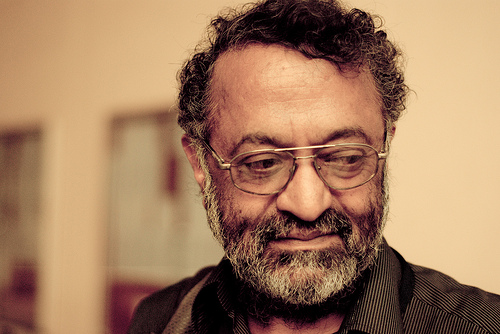
\includegraphics[height=5cm]{kenneth.jpg}
   \end{center}

  \end{block}


\end{frame}

\begin{frame}
 \frametitle{About}

\end{frame}

\begin{frame}
 \frametitle{Purpose}
\begin{block}{}
 \begin{itemize}
  \item Learn art of computer programming with one of the easiest programming language in the world.
  \item Get ready to enjoy the joy of programming in Python.
 \end{itemize}

\end{block}

\end{frame}

\begin{frame}
 \frametitle{Warning}
  \begin{itemize}
   \item This is a hands on training program.
   \item No theory included in the slides; it may discussed whenever and wherever it is required.
   \item Be patient,listen, practice and ask questions
   \item Do not hesitate to experiment 
   \item Our volunteers are here to help you in practising
   \item Be courageous enough to try 
   \item We are leaning Python not rocket science
   \item Be simple and think in a simplistic way
  \end{itemize}

\begin{alertblock}{}
Are You Ready !
\end{alertblock}


\end{frame}

\begin{frame}
 \frametitle{Why Python}
\begin{alertblock}{Why }
\begin{itemize}
 \item Used almost everywhere 
 \item Fun
 \item Concise
 \item Simple
 \item Powerful 
 \item Filled with spices to write effective programs
\end{itemize}

\end{alertblock}
\end{frame}


\begin{frame}
 \frametitle{Installation}
 \begin{block}{}
  Already installed in GNU/Linux systems \\
  If you are using M\$ Windows download Python from python.org \\
  If you are downloading Python for Windows remember to download Python 2.7 only.
 \end{block}
  
\end{frame}

\begin{frame}
 \begin{alertblock}{}
  \begin{center}
     Interactive Interpreter
  \end{center}
 \end{alertblock}

\end{frame}

\begin{frame}
 \frametitle{Interpreter}
  \begin{block}{Contains REPL}
  \begin{itemize}
   \item Read
   \item Evaluate
   \item Print
   \item Loop
  \end{itemize}

   
  \end{block}

\end{frame}

\begin{frame}
 \frametitle{Interpreter}
 %\includegraphics[height=1cm]{hw1.png}
 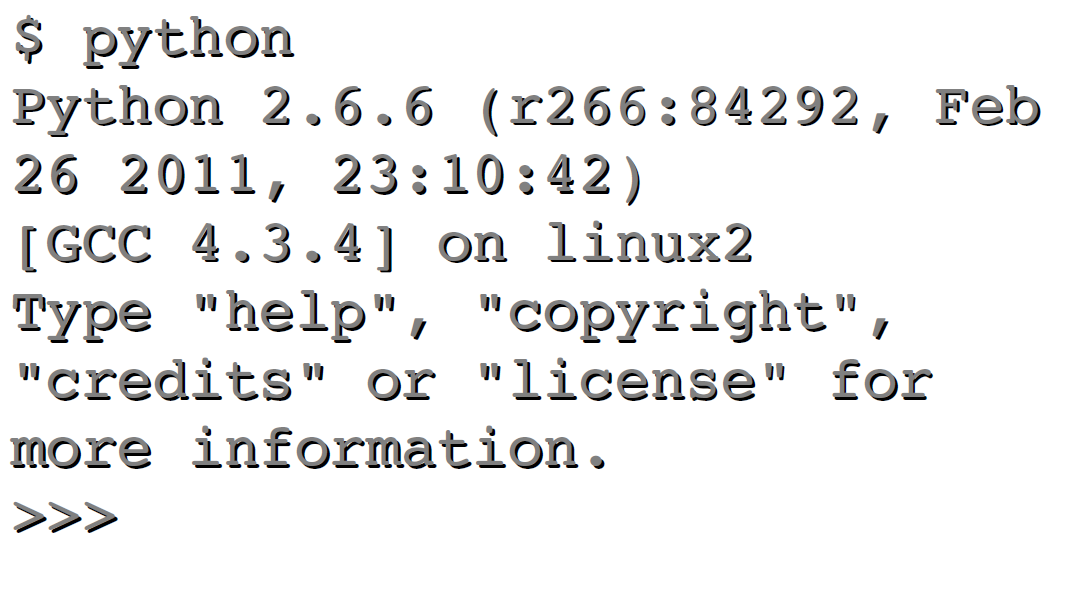
\includegraphics[height=5cm]{Inter.png}
\end{frame}

\begin{frame}[fragile]
 \frametitle{Hello World!!}
 \begin{block}<+->{Why Hello World}
  Writing 'Hello World' program is the ritual to please the programming gods to be a good programmer!!
 \end{block}
 
\begin{verbatim}
  >>> print "Hello World"
  Hello world
\end{verbatim}

\end{frame}

\begin{frame}[fragile]
 \frametitle{Let's Jump to Programming}
 \begin{center}
  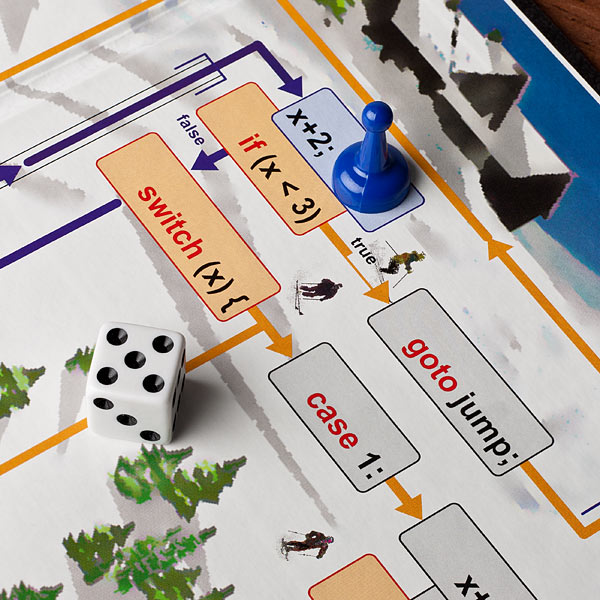
\includegraphics[height=6cm]{jump.jpg}
 \end{center}

\end{frame}

\begin{frame}[fragile]
 \frametitle{Programming Practice - 1}
 Create a file hello.py \\
 type \color{green} print \color{red}''Hello World'' \\
 \color{blue} Listen to the screen for instructions. \\
 In-case of any issues just raise your hand our volunteers will be there to help you.
\end{frame}

\begin{frame}[fragile]
 \frametitle{Programming Practice - 1}
 Run the program
 \begin{verbatim}
  $python hello.py
 \end{verbatim}

\end{frame}

\begin{frame}[fragile]
 \frametitle{Time to make your hands dirty}
 \begin{block}<+->{Note}
  Make sure that you have understood the first step.\\
  In-case of trouble we can practice it for couple of minutes.
 \end{block}
\end{frame}

\begin{frame}[fragile]
 \frametitle{Variables}
 \begin{verbatim}
  age = 33                # Integer
  avg = 33.35             # Float
  name = "linux"          # String
  bool = True             # Boolean
  another = "44"          # String
 \end{verbatim}

\end{frame}

\begin{frame}[fragile]
 \frametitle{Variables - naming}
 \begin{itemize}
  \item use lowercase
  \item use underscore between words  my\_age
  \item do not start with numbers
  \item do not use built-ins
  \item do not use keywords
 \end{itemize}

\end{frame}

\begin{frame}
 \frametitle{Reserved}
 \color{red}
and       del       for       is        raise     
assert    elif      from      lambda    return   
break     else      global    not       try     
class     except    if        or        while  
continue  exec      import    pass      yield 
def       finally   in        print
\end{frame}

\begin{frame}
 \frametitle{Time to make your hands dirty}
 \begin{center}
  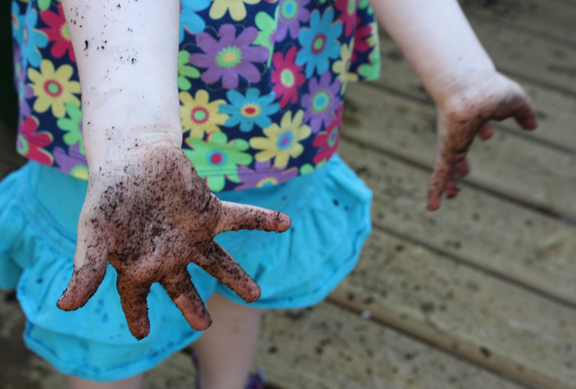
\includegraphics[height=6cm]{hd.jpg}
 \end{center}
\end{frame}

\begin{frame}[fragile]
 \frametitle{Everything is an object}
 \begin{itemize}
  \item Everything in python is an object 
 \end{itemize}
 \begin{block}<+->{An object has}
  \begin{itemize}
   \item identity (id)
   \item type (type)
   \item value (mutable or immutable)
  \end{itemize}
 \end{block}
 \begin{verbatim}
  >>> age = 33
  >>> type(age)
  <type 'int'>
  >>> id(age)
  167263248
  >>> age 34
  >>> id(age)
  167263236
 \end{verbatim}

\end{frame}

\begin{frame}[fragile]
 \frametitle{Casting}
 \begin{center}
   
\includegraphics[height=2cm]{cast.png}
 \begin{verbatim}
  >>> age = 33
  >>> str(age)
  '33'
  >>> float(age)
  33.0
  >>> long(age)
  33L
  >>> int(age)
  33
 \end{verbatim}
 \end{center}
\end{frame}

\begin{frame}
 \frametitle{Time for some maths}
 \begin{block}{}
  + , - , * , ** (power),\% (modulo), // (floor division), $<$ (less than) \\
  $>$ greater than, $<=$, $>=$, $==$ 
 \end{block}

\end{frame}

\begin{frame}
 \frametitle{It is maths time now}
 \begin{center}
  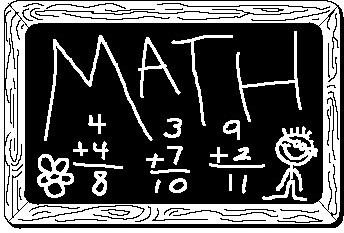
\includegraphics[height=7cm]{math.jpg}
 \end{center}

\end{frame}

\begin{frame}[fragile]
 \frametitle{String}
 \begin{verbatim}
  >>> name = 'linux'
  >>> address = "Coimbatore 1st street"
  >>> description = """ We are teaching python to 
  young chaps"""
  >>> with_new = "this sentence have one \n new line"
 \end{verbatim}

\end{frame}

\begin{frame}[fragile]
 \frametitle{String}
 \begin{verbatim}
  >>> name = "linux"
  >>> nameu = name.upper()
  >>> namel = nameu.lower()
  >>> namel.find('l')
  >>> ",".join(name)
  >>> name.startswith('l')
  >>> name.endswith('x')
  >>> namet = name.title()
  >>> wspace = "     with space "
  >>> stripped = wspace.strip()
 \end{verbatim}

\end{frame}

\begin{frame}
 \frametitle{Playing with String}
 \begin{center}
  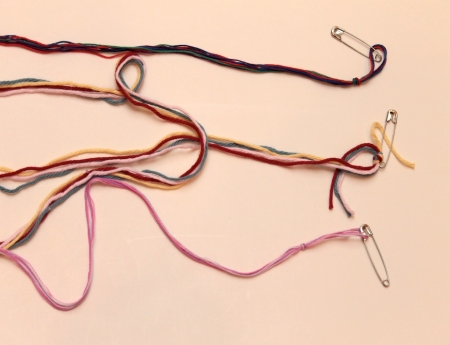
\includegraphics[height=6cm]{string.jpg}
 \end{center}
\end{frame}

\begin{frame}[fragile]
 \frametitle{Comments}
 \begin{itemize}
  \item Single line comments starts with \#
  \item Multi-line comments should be with in """ """
   \end{itemize}
\begin{verbatim}
   >>> avg = 45.34 #float
   >>> name = "ilug-cbe" """ This is a 
   multiline comment """
  \end{verbatim}
\end{frame}

\begin{frame}[fragile]
 \frametitle{Boolean}
\begin{center}
  \begin{verbatim}
  >>> t = True
  >>> f = Flase
  
  >>> n = None
 \end{verbatim}
\end{center}

\end{frame}


\begin{frame}[fragile]
 \frametitle{Conditionals}
 \begin{block}{equality,greater,less,is, is not ...}
 $==$, $!=$, $>$, $>=$, $<$, $<=$, is, is not
 \end{block}

\end{frame}

\begin{frame}[fragile]
 \frametitle{Conditionals}
 \begin{verbatim}
  >>> 1 == 1
  >>> 1 >= 0
  >>> 0 <= 1
  >>> 0 != 1
  >>> "Rajani" is "rajani"
  >>> "Vijay" is not "Rajani"
  >>> name = None
  >>> if name is not None:
  ...     #do something
 \end{verbatim}

\end{frame}

\begin{frame}[fragile]
 \frametitle{Boolean operators}
 Used to combine conditional logic
 \begin{itemize}
  \item and
  \item or
  \item not
 \end{itemize}

\end{frame}

\begin{frame}[fragile]
 \frametitle{if ...}
 \begin{verbatim}
  if mark > 60 and mark < 100:
    print "First Class"
  elif mark < 60:
    print "Second Class Only :-("
  else:
    print "Ooops !!!!"
 \end{verbatim}

\end{frame}

\begin{frame}
 \frametitle{if ... elif time }
 
\includegraphics[height=6cm]{ifelse.jpg}
\end{frame}

\begin{frame}[fragile]
 \frametitle{Sequences}
 \begin{block}{list}
  List is an ordered collection of objects.
 \end{block}
 \begin{verbatim}
  names = ["rms","linus","guido","larry"]
  marks = [45,50,60,80,90]
  mixed = ["linux",12,12.35,90L]
 \end{verbatim}
\end{frame}

\begin{frame}[fragile]
 \frametitle{Sequences - list}
 \begin{verbatim}
  names = []
  print names
  names.append("linus")
  print names
  numbers = [6,9,2,3,1,8,4]
  print len(numbers)
  print numbers.sort()
  print numbers.reverse()
  another = [9,3,6]
  numbers.extend(another)
  print numbers
  numbers.insert(0,20)
  print numbers
 \end{verbatim}

\end{frame}


\begin{frame}[fragile]
 \frametitle{Sequences - list}
 \begin{verbatim}
  print numbers[0]
  print numbers[-1]
  print numbers[2:-2]
  print numbers[:-2]
  print numbers[2:]
  print numbers[:]
 \end{verbatim}
\end{frame}

\begin{frame}[fragile]
 \frametitle{Sequences -tuple}
 \begin{block}{tuple}
  Tuple is like list only. But tuple is immutable
 \end{block}
 \begin{verbatim}
  nums = (1,2,3,4)
  print nums
  print len(nums)
  print nums[0]
  print nums[-1]
 \end{verbatim}
\end{frame}

\begin{frame}[fragile]
 \frametitle{Sequences range}
 \begin{verbatim}
  nums = range(20)
  print nums
  selected = range(20,60)
  print selected
  jump2 = range(10,100,2)
  print jump2
 \end{verbatim}

\end{frame}

\begin{frame}[fragile]
 \frametitle{Let's do some sequencing}
 \begin{center}
  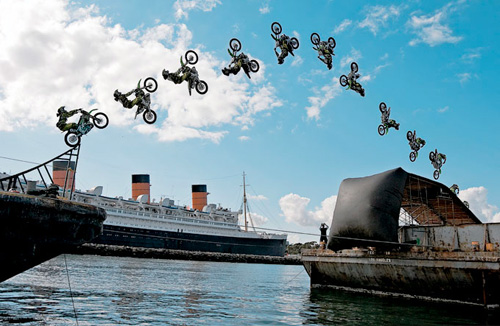
\includegraphics[height=6cm]{seq.jpg}
 \end{center}

\end{frame}


\begin{frame}[fragile]
 \frametitle{Iteration}
 \begin{verbatim}
  names = ["linus","rms","guido","larry"]
  for name in names:
    print "hello %s" %(name)
  
  for num in range(10,20,2):
    print num
   
 \end{verbatim}

\end{frame}

\begin{frame}[fragile]
 \frametitle{Iteration}
 \begin{verbatim}
  for i in range(len(names)):
    print i,names[i]
  
  for i,v in enumerate(names):
    print i,v
 \end{verbatim}

\end{frame}

\begin{frame}[fragile]
 \frametitle{Iteration break,continue and pass}
 \begin{verbatim}
  for name in names:
    print name
    if name == "guido":
      break
  
  
  for name in names:
    print name
    if name == "linus":
      continue
  
  for name in names:
    print name
    if name == "rms":
      pass
 \end{verbatim}

\end{frame}

\begin{frame}[fragile]
 \frametitle{Iteration - while}
 \begin{verbatim}
  my_number = 10
  
  while my_number < 20:
     print my_number
     my_number += 2
 \end{verbatim}

\end{frame}


\begin{frame}[fragile]
 \frametitle{Let's Iterate}
 \begin{center}
  
\includegraphics[height=6cm]{iter.jpg}
 \end{center}

\end{frame}

\begin{frame}[fragile]
 \frametitle{Dictionaries}
 Also called as hash, hashmap or associative array
 \begin{verbatim}
  address = {"name":"ILUG-CBE","houseno":"Nil",
  "street":"any whare","city":"Coimbatore"}
  print address
  
 \end{verbatim}

\end{frame}

\begin{frame}[fragile]
 \frametitle{Dictionaries}
 \begin{verbatim}
  address["state"] = "tamilnadu"
  address["web"] = "ilugcbe.org.in"
  
  print address
 \end{verbatim}

\end{frame}

\begin{frame}[fragile]
 \frametitle{Dictionaries}
 \begin{verbatim}
  print address.has_key("country")
  
  print address.get("phone","No Phone Number Provided")
 \end{verbatim}

\end{frame}


\begin{frame}[fragile]
 \frametitle{Dictionaries}
 \begin{verbatim}
  address.setdefault("country","India")
  
  print address
  
  print address.keys()
  
  print address.values()
  
  print address.items()
  
  del address["country"]
  
  print address
 \end{verbatim}

\end{frame}

\begin{frame}[fragile]
 \frametitle{Let's practice Dictionaries}
 
\includegraphics[height=6cm]{dict.jpg}
\end{frame}

\begin{frame}[fragile]
 \frametitle{Functions}
 \begin{verbatim}
  def say_hai():
    print "hello"
  
  say_hai()
 \end{verbatim}

\end{frame}

\begin{frame}[fragile]
 \frametitle{Functions}
 \begin{verbatim}
  def add_two(num):
    return num + 2
  
  res = add_two(4)
  
  print res
 \end{verbatim}

\end{frame}

\begin{frame}[fragile]
 \frametitle{Functions}
 \begin{verbatim}
  def add(a,b):
    """
    adds two numbers
    """ 
    return a + b
  
  res = add_two(4,5)
  
  print res
 \end{verbatim}

\end{frame}

\begin{frame}[fragile]
 \frametitle{Functions}
 \begin{verbatim}
  def demo(*args):
    """
    *args demo
    """ 
    for arg in args:
      print i * 2
  
  demo(1,2,3,4,5,6)
 \end{verbatim}

\end{frame}

\begin{frame}[fragile]
 \frametitle{Functions}
 \begin{verbatim}
  def demo(num,*args):
    """
    *args demo
    """ 
    for arg in args:
      print i * num
  
  demo(1,2,3,4,5,6)
 \end{verbatim}

\end{frame}

\begin{frame}[fragile]
 \frametitle{Functions}
 \begin{verbatim}
  def demo(num,*args):
    """
    *args demo
    """ 
    mul = []
    for arg in args:
      mul.append(i * num)
    
    return sum(mul)
  
  res = demo(2,2,3,4,5,6)
  
  print res
 \end{verbatim}

\end{frame}

\begin{frame}[fragile]
 \frametitle{Functions}
 \begin{verbatim}
  def marker(roll_no,details):
    if details['marks'] > 60:
      print "Roll no %d %s" %(roll_no, "First Class")
  
  marker(12,marks = 62)
 \end{verbatim}

\end{frame}

\begin{frame}[fragile]
 \frametitle{Functions}
 \begin{verbatim}
  def mulbythree(num,three=3):
    """
    default argument example
    """
    return num * three
  
  res = mulbythree(43)
  print res
 \end{verbatim}

\end{frame}

\begin{frame}
 \frametitle{Be functional now}
 \begin{center}
  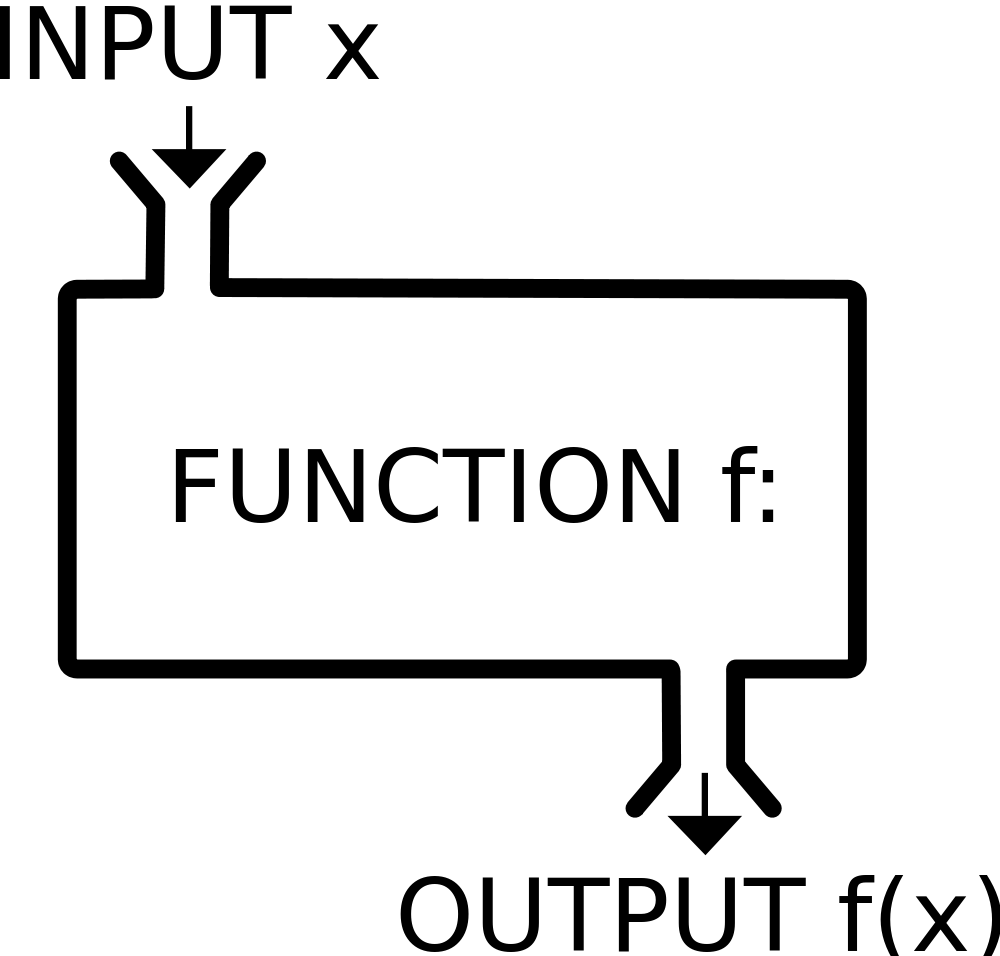
\includegraphics[height=7cm]{fun.png}
 \end{center}

\end{frame}

\begin{frame}[fragile]
 \frametitle{Tricks 1}
 \begin{verbatim}
  nums = [1,2,3,4,5,6,7,8,9]
  mulbt = [num * 2 for num in nums]
  
  print nums
  print mulbt
 \end{verbatim}

\end{frame}

\begin{frame}[fragile]
 \frametitle{Tricks - 2}
 \begin{verbatim}
  nums = [1,2,3,4,5,6,7,8,9]
  mulbt = [num * 2 for num in nums if num / 2 != 0]
  
  print nums
  print mulbt
 \end{verbatim}

\end{frame}

\begin{frame}[fragile]
 \frametitle{Tricks - 3}
 \begin{verbatim}
  nums = [1,2,3,4,5,6,7,8,9]
  numtuple = tuple(nums)

  print type(nums)
  print type(numtuple)
 \end{verbatim}

\end{frame}

\begin{frame}[fragile]
 \frametitle{Tricks - 4}
 \begin{verbatim}
  print "ILUGCBE".lower().upper().title()
 \end{verbatim}

\end{frame}

\begin{frame}[fragile]
 \frametitle{User input}
 \begin{verbatim}
  name = raw_input("Tell your name: ")
  
  print name
  
  age = int(raw_input("Tell your age: "))
  
  print age
  
 \end{verbatim}

\end{frame}

\begin{frame}
 \frametitle{Tricks time }
 \begin{center}
  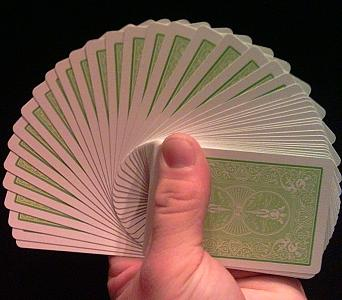
\includegraphics[height=7cm]{trick.jpg}
 \end{center}

\end{frame}


\begin{frame}[fragile]
 \frametitle{Lambda}
 %sum = lambda x, y:   x + y   #  def sum(x,y): return x + y
 \begin{verbatim}
  product = lambda x,y : x * y
  
  res = product(12,13)
  print res
 \end{verbatim}

\end{frame}

\begin{frame}[fragile]
 \frametitle{Lambda}
 %sum = lambda x, y:   x + y   #  def sum(x,y): return x + y
 \begin{verbatim}
  dbtnt = lambda x : x * 2 if x % 2 == 0 else x
  
  res = dbtnt(12)
  print res
 \end{verbatim}

\end{frame}

\begin{frame}[fragile]
 \frametitle{Lambda}
 %sum = lambda x, y:   x + y   #  def sum(x,y): return x + y
 \begin{verbatim}
  bors = lambda x: x > 100 and 'big' or 'small'
  
  for i in (1, 10, 99, 100, 101, 110):
      print i, 'is', bors(i)
  
 \end{verbatim}

\end{frame}

\begin{frame}[fragile]
 \frametitle{Object Oriented Programming - basics}
  \begin{verbatim}
   class MyClass:
       """
       This is my class
       """
       def __init__(self):
           #nothing

       def say_hai(self):
           print "Hai"
    
    obj = MyClass()
    obj.say_hai()
  \end{verbatim}

\end{frame}

\begin{frame}[fragile]
 \frametitle{Object Oriented Programming - basics}
  \begin{verbatim}
   class MyClass(object):
       """
       This is my class
       """
       def __init__(self):
           #nothing

       def say_hai(self):
           print "Hai"
    
    obj = MyClass()
    obj.say_hai()
  \end{verbatim}

\end{frame}

\begin{frame}[fragile]
 \frametitle{Object Oriented Programming - basics}
  \begin{verbatim}
   class Student:
       """
       Student class
       """

       def __init__(self):
           self.college = "My College"

       def greet(self,name):
           """
           Function to greet student
           """
           print "Hello %s from %s" %(name, self.college)
 
    student = Student()
    student.greet("Jaganadh")
  \end{verbatim}

\end{frame}

\begin{frame}[fragile]
 \frametitle{Object Oriented Programming - inheritance}
  \begin{verbatim}
   class BeStudent:
       def __init__(self):
           Student.__init__(self)
           self.class = "BE First Year"

       def greet(self,name):
           print "Hello %s from %s %s class" %(name,
           self.college,self.class)

    student = BeStudent()
    student.greet("Jaganadh G")
  \end{verbatim}

\end{frame}

\begin{frame}
 \frametitle{Object Oriented Time}
\begin{center}
 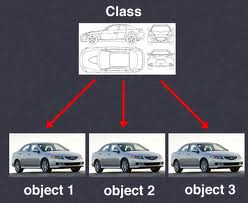
\includegraphics[height=6cm]{oops.jpeg}
\end{center}

\end{frame}

\begin{frame}[fragile]
 \frametitle{File I/O - read file}
  \begin{verbatim}
  input = open("file.txt",'r')
  contents = input.read()
  input.close()

  print contents

  input = open("file.txt",'r')
  contents = input.readlines()
  input.close()

  print contents
  
  \end{verbatim}

\end{frame}

\begin{frame}[fragile]
 \frametitle{File I/O - write to file}
  \begin{verbatim}
  names = ["linus","rms","larry","guido"]
  output = open("out_file.txt",'w')
  for name in names:
      output.write(name)
      output.write("\n")

  \end{verbatim}

\end{frame}

\begin{frame}[fragile]
 \frametitle{File I/O - write to file}
  \begin{verbatim}
  names = ["linus","rms","larry","guido"]
  output = open("out_file.txt",'a')
  for name in names:
      output.write(name)
      output.write("\n")

  \end{verbatim}

\end{frame}

\begin{frame}
 \frametitle{Let's play with files}
\begin{center}
 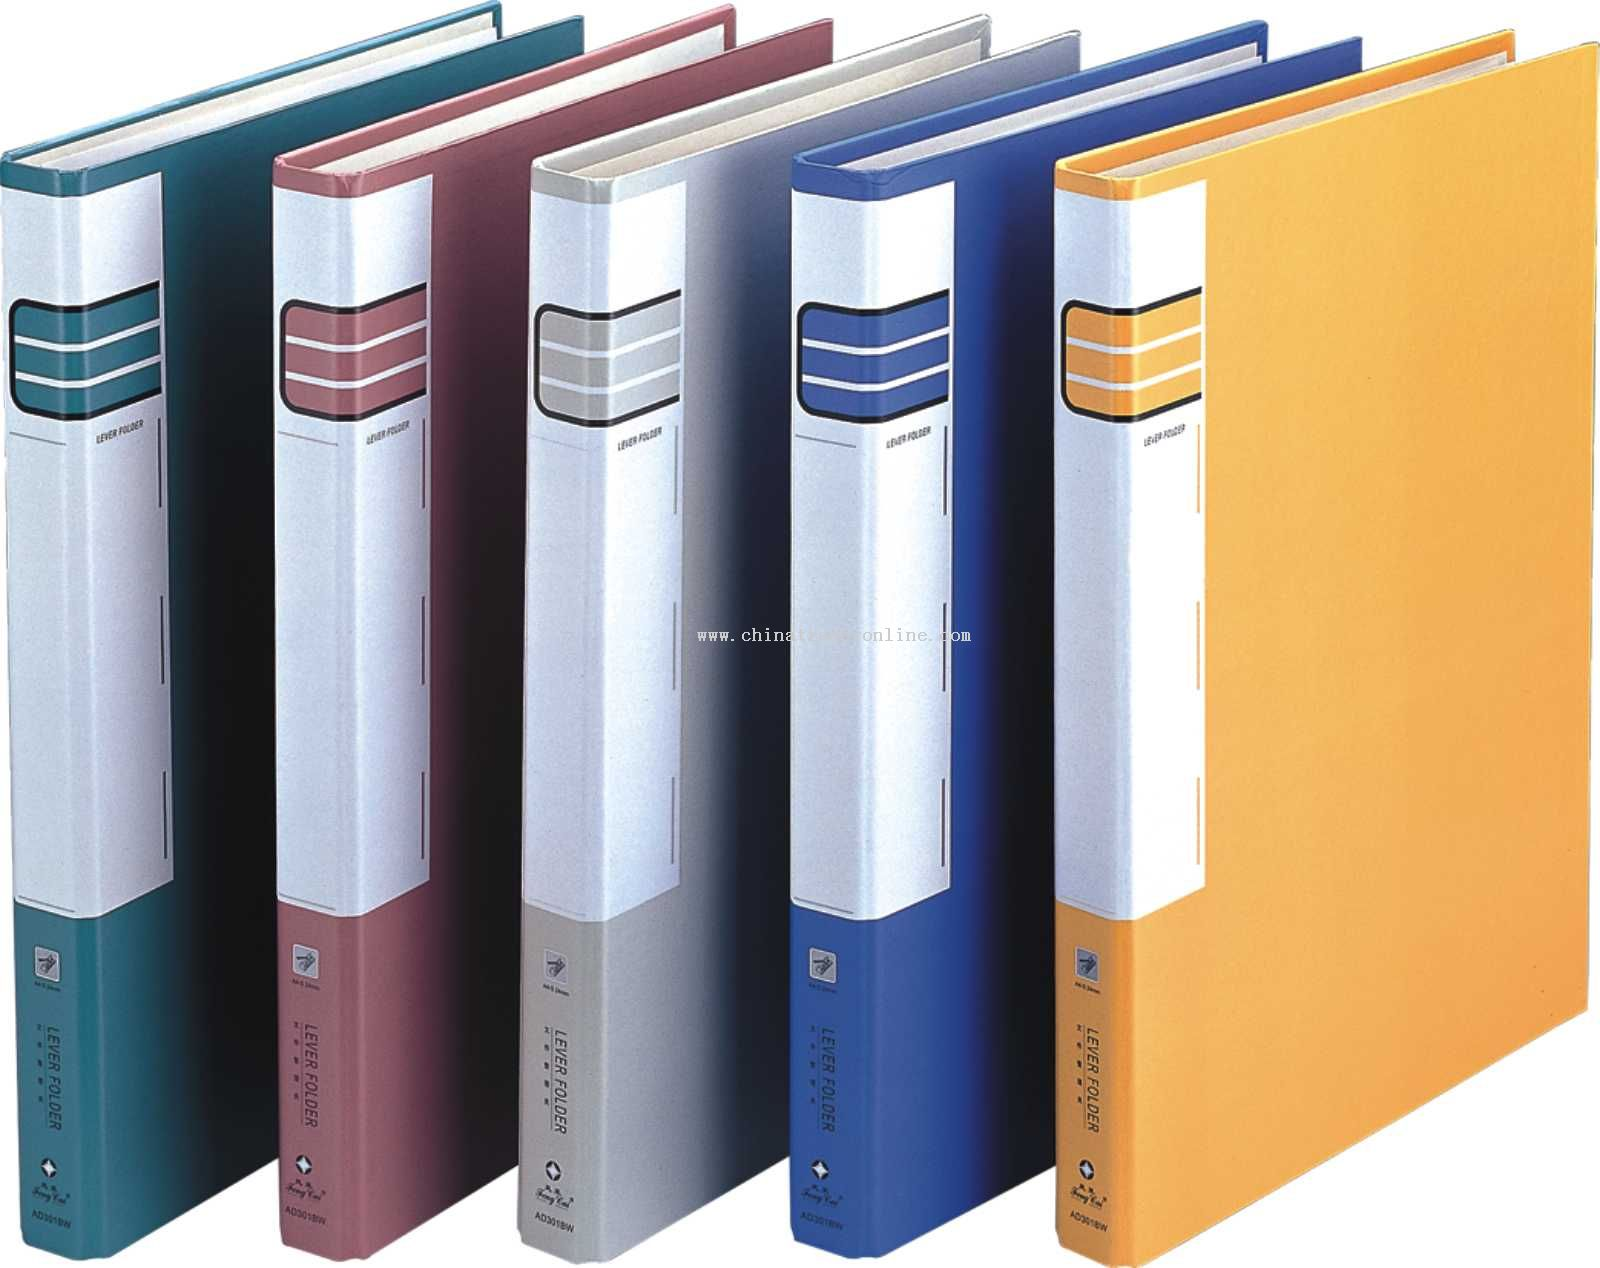
\includegraphics[height=6cm]{file.jpg}
\end{center}

\end{frame}


\begin{frame}[fragile]
 \frametitle{Batteries}
  \begin{block}{Standard Libraries}
   Python comes with batteries included. Lots of useful libraries are there in the language. Let's see some of these libraries now
  \end{block}

  \begin{verbatim}
   import math
   print math.pi
   print math.sqrt(10)
   print math.factorial(10)
   print math.sin(10)
   print math.pow(10,2)
   print math.log(10)
   print math.log(10,2)
   print math.log10(10)
   print math.exp(10)
  \end{verbatim}

\end{frame}

\begin{frame}[fragile]
 \frametitle{Batteries - sys}
\begin{verbatim}
 import sys
 print sys.platform
 
 afl = sys.argv[1]

 print sys.version
 print sys.maxint
 print sys.maxsize
\end{verbatim}

\end{frame}

\begin{frame}[fragile]
 \frametitle{Batteries - os}
\begin{verbatim}
 import os
 print os.curdir()
 print os.getlogin()
 print os.getcwd()
 print os.name
\end{verbatim}

\end{frame}

\begin{frame}[fragile]
 \frametitle{Batteries - time,random}
\begin{verbatim}
 import time
 print time.ctime()
 print time.gmtime()
 
 import random
 print random.random()
 print random.choice([1,2,3,4,5,6]) 
\end{verbatim}

\end{frame}

\begin{frame}
 \frametitle{Battery Recharge}
\begin{center}
 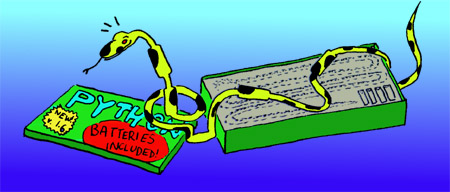
\includegraphics[height=5cm]{batt.jpg}
\end{center}

\end{frame}

\begin{frame}
 \frametitle{Question Time}
\begin{center}
 
\includegraphics[height=6cm]{ques.jpg}
\end{center}

\end{frame}

\begin{frame}
 \frametitle{Contributors}
\begin{center}
 \begin{itemize}
  \item Jaganadh G           @jaganadhg
  \item Biju B               @bijubk
  \item Satheesh Kumar D     
  \item Sreejith S           @tweet2sree
  \item Rajith Ravi          @chelakkandupoda
 \end{itemize}

\end{center}

\end{frame}

\begin{frame}
 \frametitle{Contact US}
\begin{block}{Web}
 http://ilugcbe.org.in \\
 mail mail2ilugcbe@gmail.com
\end{block}

\end{frame}

\begin{frame}
 \frametitle{References}
\begin{itemize}
 \item A Byte of Python, CH Swaroop, http://www.swaroopch.org/notes/Python
 \item Hands on Beginning Python,Matt Harrison,http://cdn.oreillystatic.com/en/assets/1/event/61/Hands on Beginning Python Presentation.gzip
 \item Learning Python,Mark Lutz, David Ascher,http://shop.oreilly.com/product/9781565924642.do
 \item Beginning Python From Novice to Professional,Magnus Lie Hetland, http://www.apress.com/9781590595190/
\end{itemize}


\end{frame}


\begin{frame}
 \frametitle{Images used in the slides were taken from }
 http://www.thinkgeek.com/product/ec05/
http://blog.dailypea.com/2012/05/19/gardening-one-of-the-best-gifts-you-can-give-a-toddler/
http://6sasho6ahmetcan6.edublogs.org/
http://www.supermama.me/en/Crafts-Playing-With-String
http://www.webdesign.org/web-programming/javascript/learning-javascript-basics-operators-if-else.5920.html
 http://haha.nu/arts/photography/action-sequence-photography/
http://nerdbusiness.com/blog/how-iterate-business-strategy-with-git
http://www.duhaime.org/LegalDictionary.aspx
 http://en.wikipedia.org/wiki/Function\_mathematics
 http://card-tricks.21ace.com/
http://multimedia.journalism.berkeley.edu/tutorials/actionscript3/object-oriented-programming/
http://airsidehackers.blogspot.in/2011/10/how-to-rename-file-extensions.html
http://www.terre-adelie.org/python.html
http://freeimagesarchive.com/img1319.search.htm
\end{frame}

%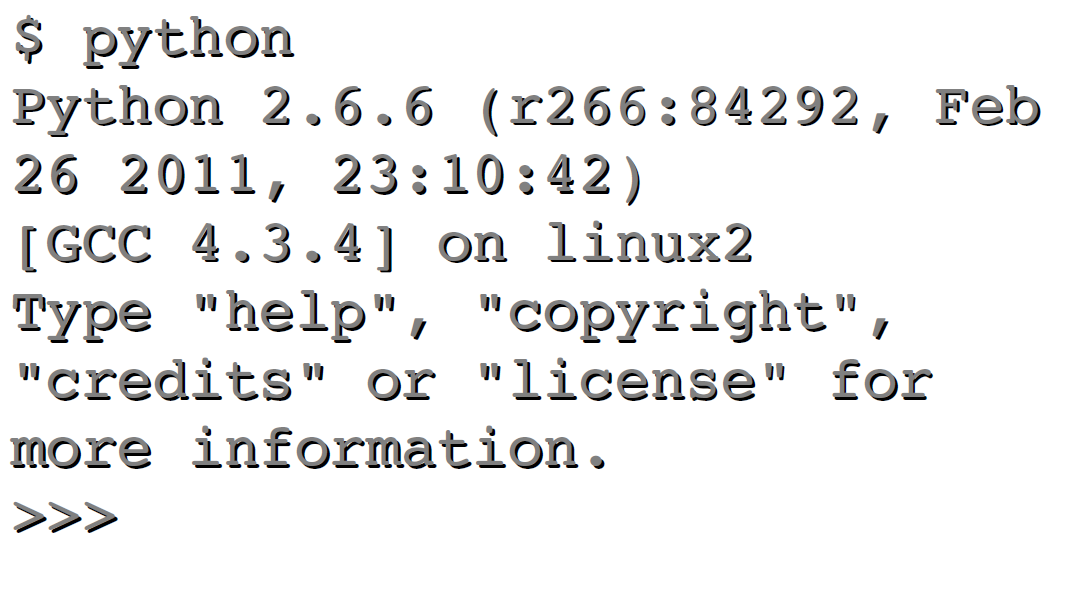
\includegraphics[height=5cm]{Inter.png}
%%%%%%%%%%%%%%%%%%%%%%%%%%%%%%%%%%%%%%%%%%%%%%%%%%%%%%%%%%%%%%%%%%%%%%%%%%%%%%%%%%%%%%%%%%%%%%%%%%%%
%Ref
%jump http://www.thinkgeek.com/product/ec05/
%HD - http://blog.dailypea.com/2012/05/19/gardening-one-of-the-best-gifts-you-can-give-a-toddler/
%math - http://6sasho6ahmetcan6.edublogs.org/
%string http://www.supermama.me/en/Crafts-Playing-With-String
%ifelse http://www.webdesign.org/web-programming/javascript/learning-javascript-basics-operators-if-else.5920.html
%seq http://haha.nu/arts/photography/action-sequence-photography/
%iter http://nerdbusiness.com/blog/how-iterate-business-strategy-with-git
%dict http://www.duhaime.org/LegalDictionary.aspx
%fun http://en.wikipedia.org/wiki/Function_%28mathematics%29
%trick http://card-tricks.21ace.com/
%oops http://multimedia.journalism.berkeley.edu/tutorials/actionscript3/object-oriented-programming/
%file http://airsidehackers.blogspot.in/2011/10/how-to-rename-file-extensions.html
%batt http://www.terre-adelie.org/python.html
%ques http://freeimagesarchive.com/img1319.search.htm
%%%%%%%%
\end{document}
